\chapter{Implementation}%Jens
Due to the agile nature of the prototype development the implementation stage begun while the design phase was still underway. This chapter describes what went into the implementation of the final prototype.

\section{Micro controllers}%Daniel
	Initially doing the implementation phase, research went into what kind of micro controller, if any, we would need to construct a working prototype. Initially we settled for an Arduino Mega 2560, but going into the production phase, we realized that an external sound source was needed. The Beaglebone Black with the Bela shield suited this purpose, and was taken in during this process.
	\subsection{Arduino}%Daniel
		The Arduino devices are a small, but versatile group of micro controller, used around the world for DIY projects\todo{Find cite}. The Arduino Mega, with the ATMEGA2560 chip is one of the more powerful variants, with a bigger EEPROM and more pins than the more commonly seen Arduino Uno. The pin amount was paramount in the decision to what micro controller was needed to control the physical interface, as the design called for a 4x5 grid of fields that should be individually activated. 
		
	\subsection{Bela}%Jens
		Due to the sound related limitations from the Arduino Mega, we decided to add a connection to a Beaglebone with a Bela shield\footnote{Bela website: \url{https://bela.io/}}. The Bela provides a broad span of audio processing opportunities to create and manipulate audio as it is compatible with Pure Data(PD). PD is a visual programming language for multimedia that can also be used to create sounds.
	
\section{Code}
	\subsection{Arduino}%Daniel
	When designing the system for the mat, it came down to three requirements:
	\begin{itemize}
		\item[-] It should be able to save the activated fields in each of the four beats (lines).
		\item[-] It should be able to save the sequences of fields in four separate segments.
		\item[-] It should be able to start playback of the previously saved segments.
	\end{itemize}
		To categorize the data and prepare it for saving on the Mega, two separate structures where made. These structures as seen in \autoref{listing:structs} are called \mintinline{cpp}{SequenceField} and \mintinline{cpp}{Segment}. SequenceField contains an \mintinline{cpp}{int} that holds the octave of the sequence, and a \mintinline{cpp}{Field} array to hold the activated fields.\\\\ The \mintinline{cpp}{Segment} structure holds a \mintinline{cpp}{SequenceField} array to contain the 4 sequences (beats), a \mintinline{cpp}{bool} to keep track of what segment is enabled, and the corresponding LED pin.
		
		\begin{listing}[H]
			\caption{The structs used to contain our data for the segments and their fields.}
			\label{listing:structs}
			\begin{minted}[frame=lines,framesep=2mm,baselinestretch=1.1,fontsize=\footnotesize,linenos]{cpp}
struct SequenceField {
  int octave = 4;
  Field activatedFields[5];
};

struct Segment {
  bool enabled = true;
  int ledPin;
  SequenceField sequence[4];
};
			\end{minted}
		\end{listing}
To save the segments and their data to persist through restarts, we make use of the onboard EEPROM. The EEPROM on the Arduino Mega can hold 4k bytes of data while our segments only take up 611 bytes of that space. Writing to the EEPROM on an Arduino is quite straightforward, we simply iterate over our \mintinline{cpp}{Segment} array, and put in into the EEPROM according to the size of our structure.
		\begin{listing}[H]
			\caption{Writing our segment data to the EEPROM}
			\label{listing:writeSegment}
			\begin{minted}[frame=lines,framesep=2mm,baselinestretch=1.1,fontsize=\footnotesize,linenos]{cpp}
void writeSegments() {
  for(int i = 0; i < amountOfSegments; i++) {
	EEPROM.put(i*sizeof(Segment), segments[i]);
  }
}
			\end{minted}
		\end{listing}
		\autoref{fig:flowchartPlayRecord} explains what happens when either the record or play buttons is pressed.
		\begin{figure}[H]
			\centering
			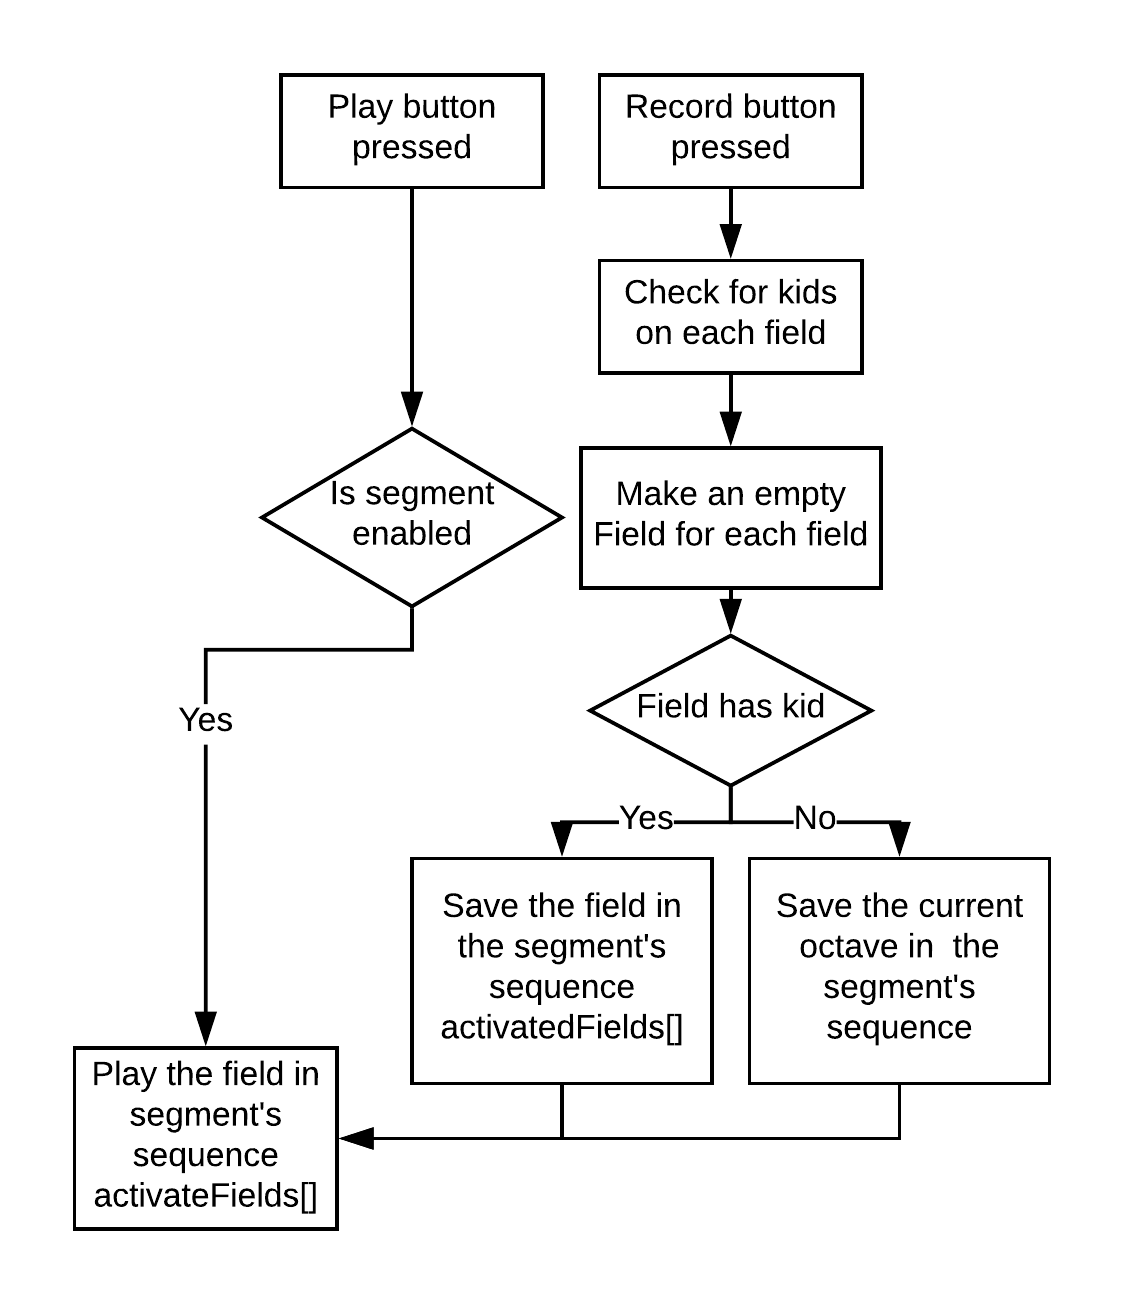
\includegraphics[width=.5\linewidth]{figure/Implementation/flowchartPlayRecord}
			\caption{Flowchart of pressing either the play or record button}
			\label{fig:flowchartPlayRecord}
			\end{figure}
	
		\subsubsection{Libraries}%Daniel
			FastLed, button.
	\subsection{PureData}%Jens
	\autoref{fig:pdPatch} shows the main patch of the PD code that was uploaded to the Bela. It takes inputs through the Belas' pins from the Arduino Mega. The PD patch is responsible for playing the sounds when the pads are pressed, changing the octave by multiplying/dividing the oscillators' frequencies by 2, playing the count in sound before recording or playing.
	
	\begin{figure}[H]
		\centering
		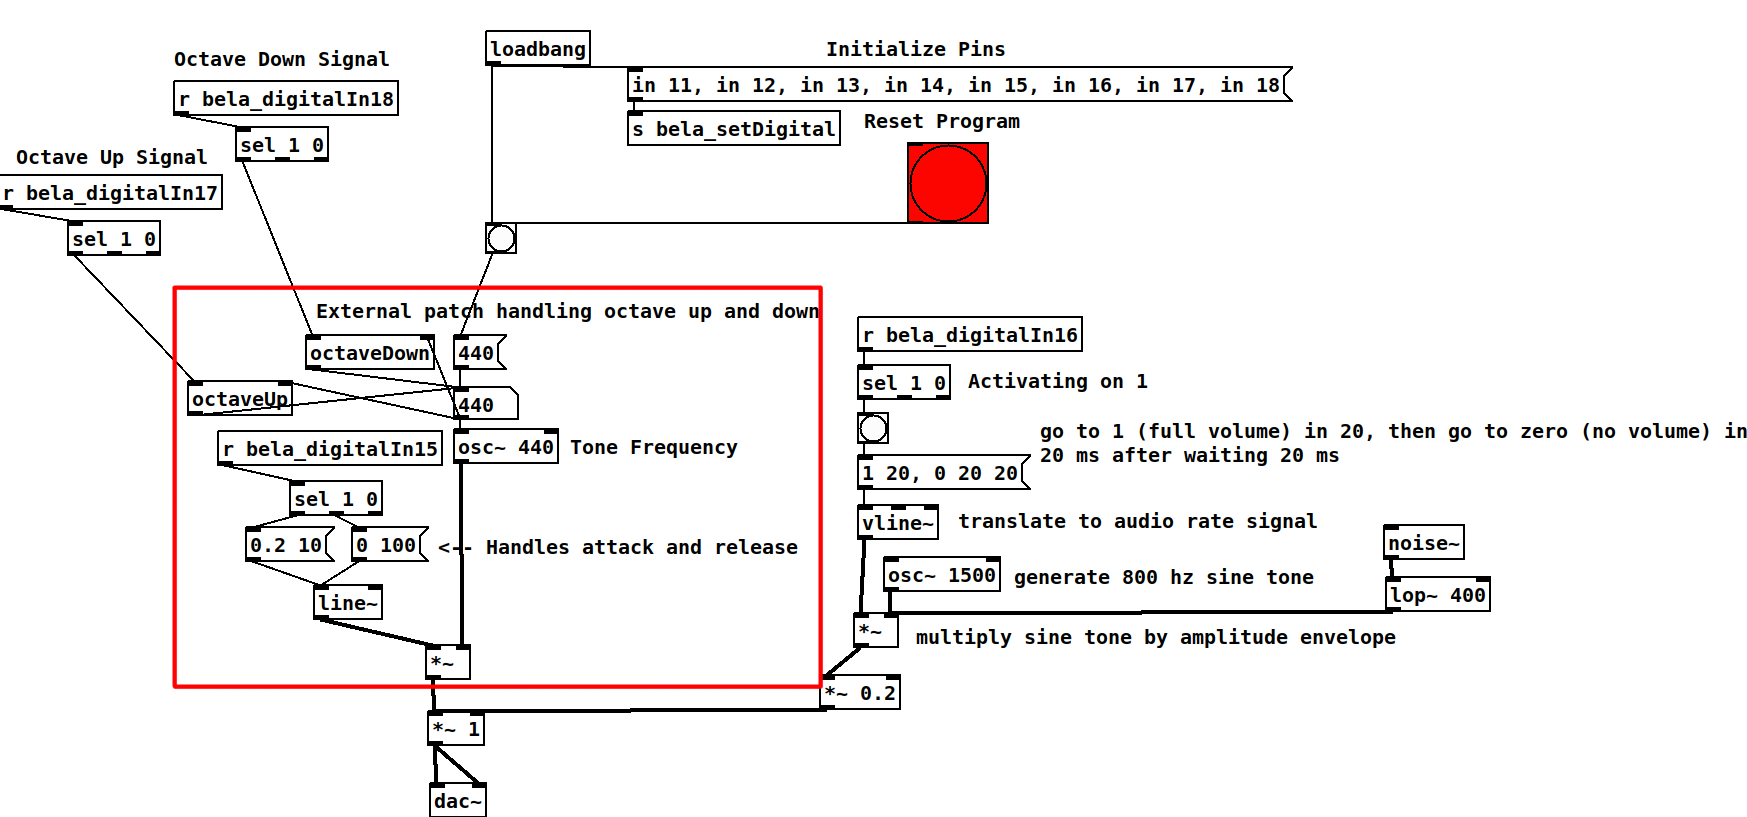
\includegraphics[width=1\linewidth]{figure/Implementation/pdPatch}
		\caption{Figure showing the main Pure Data patch for the prototype}
		\label{fig:pdPatch}
	\end{figure}
	
	Due to the 4x5 layout of the mat, and the 4 was representing 4 beats, there was a need for a scale that would fit 5 tones. Therefore a pentatonic scale was chosen. It consists of 5 tones and therefore 5 frequencies. These were generated by an Oscillator object. A functionality for octavating the scale up and down was implemented to add more variety and opportunity. By dividing the current tone frequency by 2 the octave is lowered and by multiplying by 2 it is raised. \autoref{tab:toneFreq} shows a table of the frequencies for the octaves available on the system.
	
	\begin{table}[H]
		\centering
		\caption{Table showing the oscillator tone frequencies for the pentatonic scales in the different octaves.}
		\label{tab:toneFreq}
		\begin{tabular}{|c|c|c|c|c|c|}
			\hline
			Octave/tones & C     & D     & E     & G    & A    \\ \hline
			3            & 130.5 & 146.5 & 164.5 & 196  & 220  \\ \hline
			4            & 261   & 293   & 329   & 392  & 440  \\ \hline
			5            & 522   & 586   & 658   & 784  & 880  \\ \hline
			6            & 1044  & 1172  & 1316  & 1568 & 1760 \\ \hline
		\end{tabular}
	\end{table}
	



\section{The box}%Jens
In order to conceal wires and micro controllers and to construct an easy way of controlling the various features a box was created. This section explains how the control box was built.

	\subsection{CAD}
	Autodesk's Fusion 360\footnote{Product overview page for Fusion 360: \url{https://www.autodesk.com/products/fusion-360/overview}} with an additional box generation plugin provided a convenient way of creating the blueprint for the control box that would later be used to laser cut the 6 sides of the box. Holes were cut onto the lid of the box to be able to place the needed buttons and LEDs. On the side facing the mat a square hole was cut that would be used for a custom made plug for easily connecting the mat with the Arduino Mega. For decoration a G-clef was also printed onto the front facing side (See \autoref{fig:finalbox1}). On the backside holes were cut to provide easy access for adding an external speaker through a female jack plug and also to power the Bela using a USB cable.
	
	
	\begin{figure}[H]
		\centering
		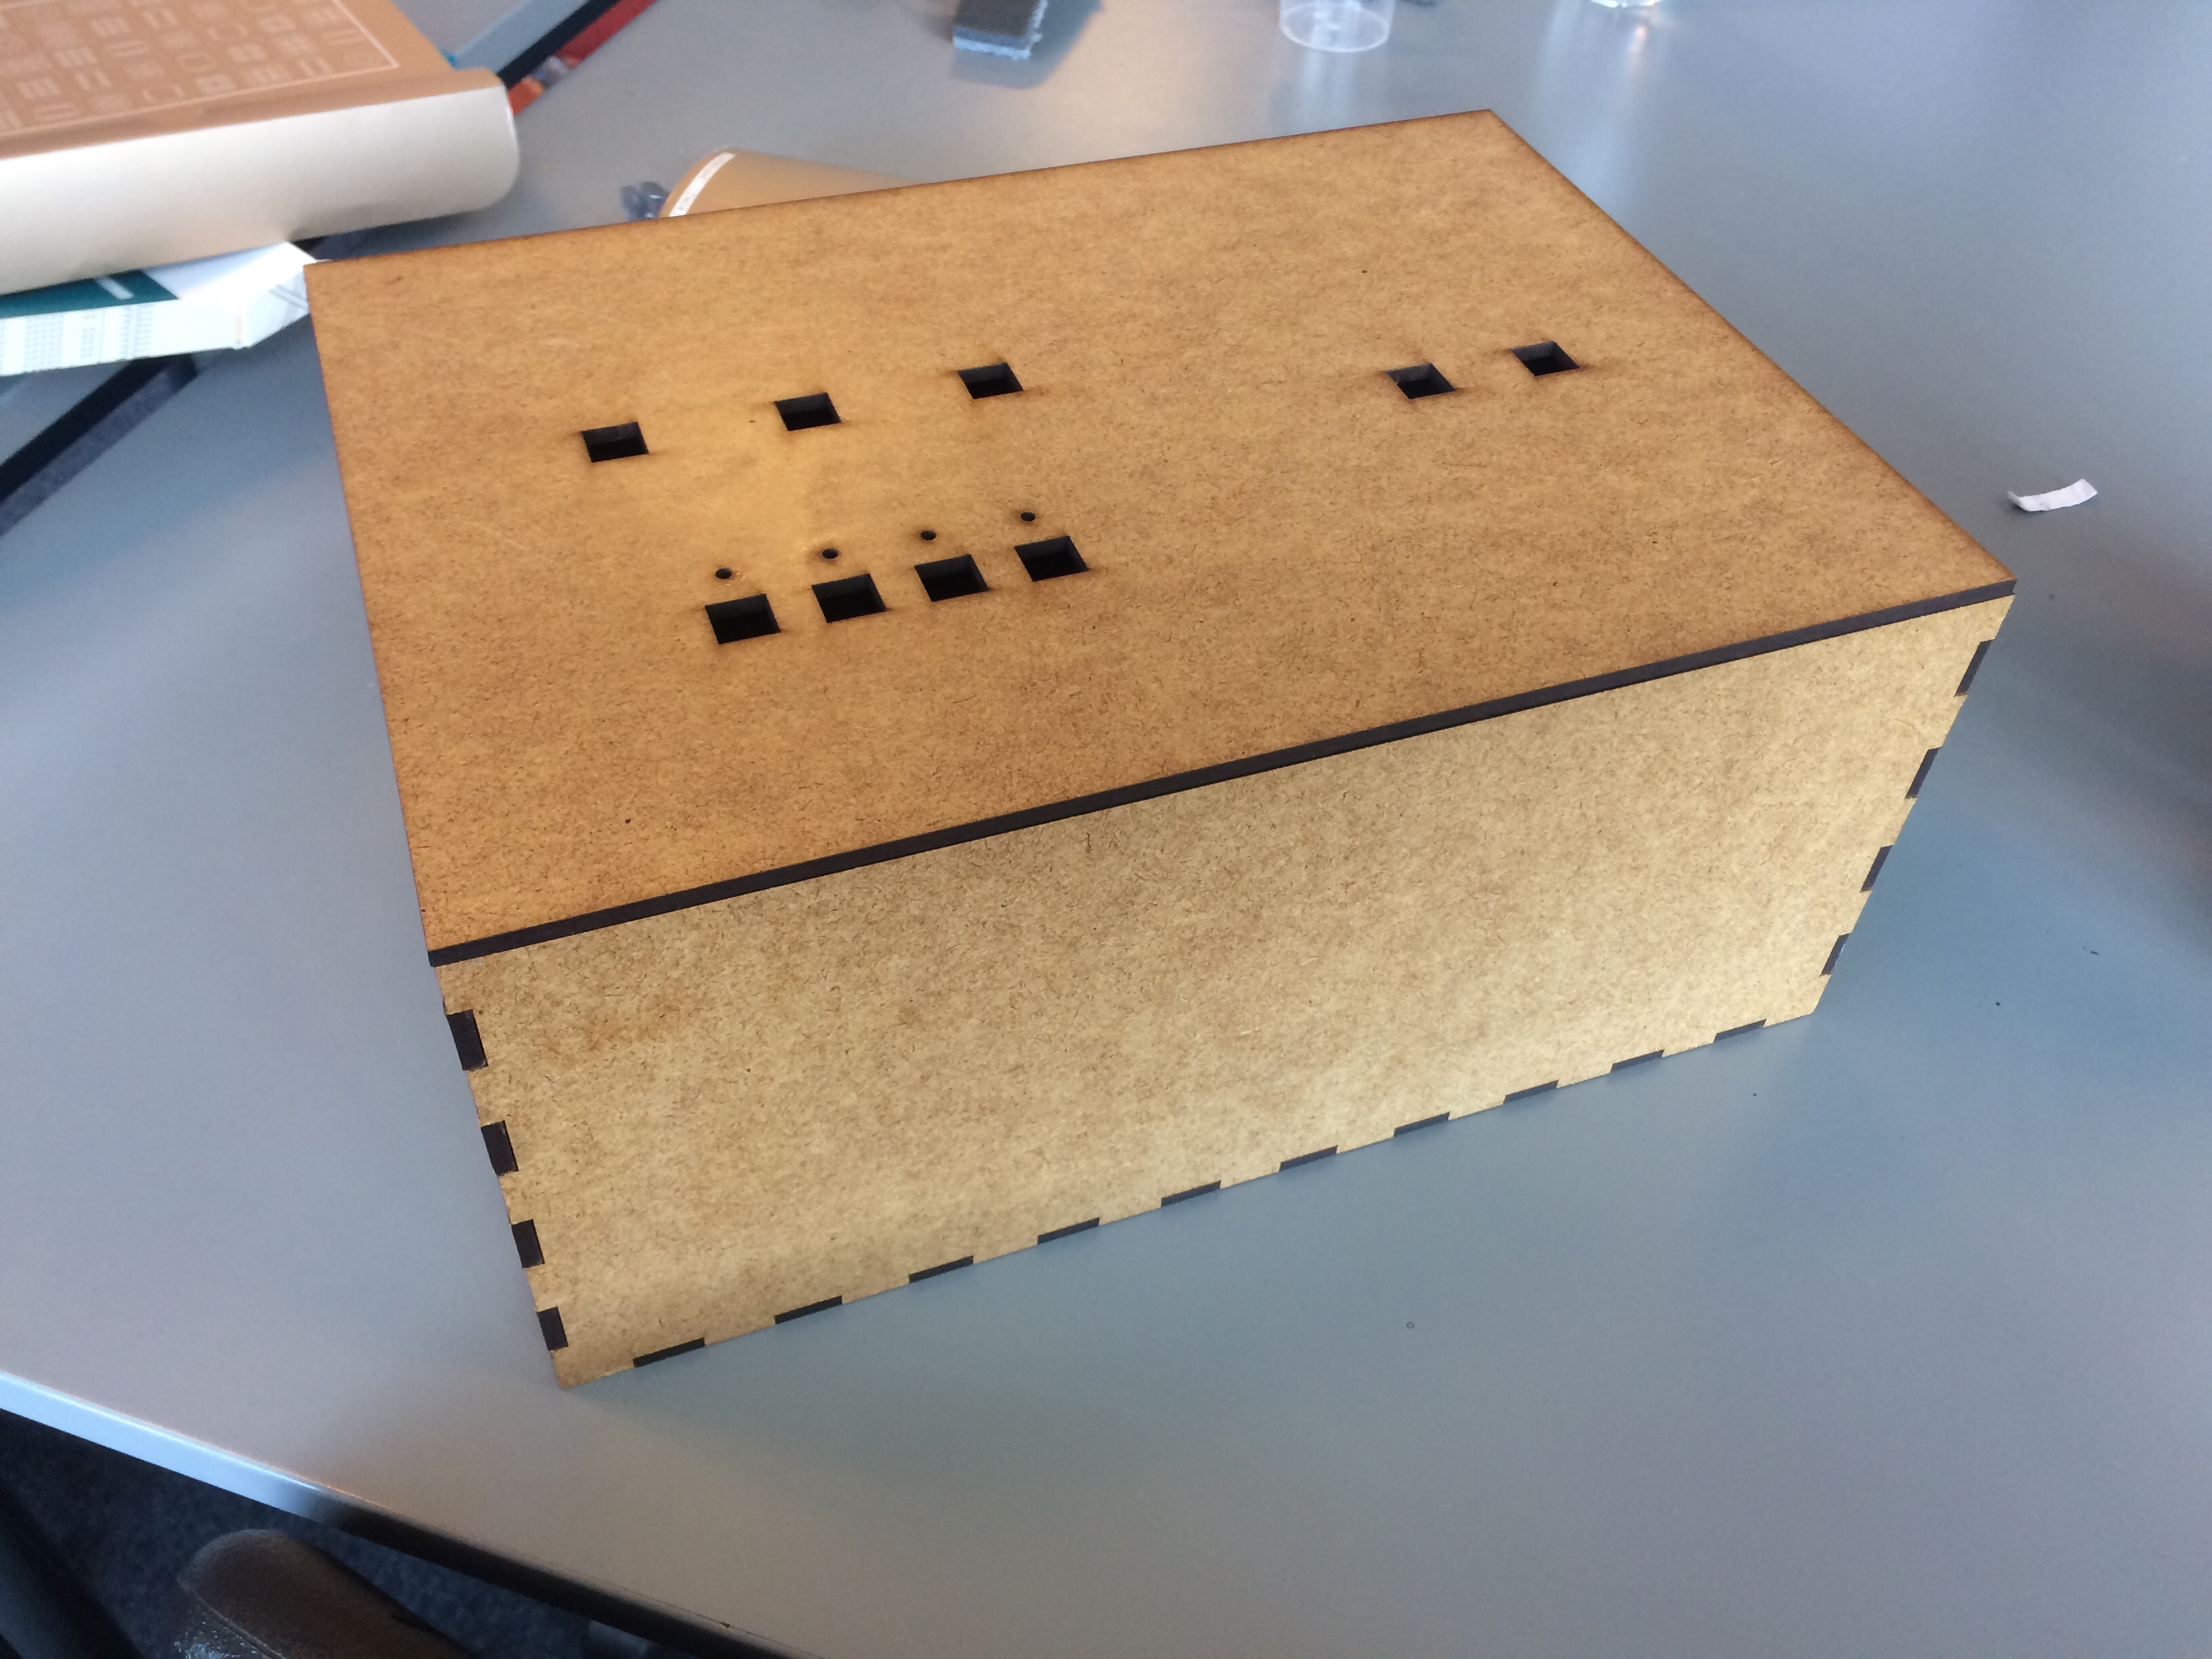
\includegraphics[width=0.7\linewidth]{figure/Design/finalbox1}
		\caption{The final prototype box}	
		\label{fig:finalbox1}
	\end{figure}
	
		
	\subsection{Assembly}
	Due to the way the sides of the box were constructed with finger joints that fit together the box was easy to assemble. With a kerf of ??\todo{What was our kerf?}mm the sides were able to stick to each other without using additional glue or nails. However, the plugs were glued to the inside of the box. This was also the case for the buttons and the LEDs on the lid. These also required wires that were soldered on with extra length which made it possible to lift the lid of the box without wires being detached from the micro controllers. Within the lid a frame was glued on to hold the lid in place since the lid was not made with joints (See \autoref{fig:finalbox2}).
	
		\begin{figure}[H]
			\centering
			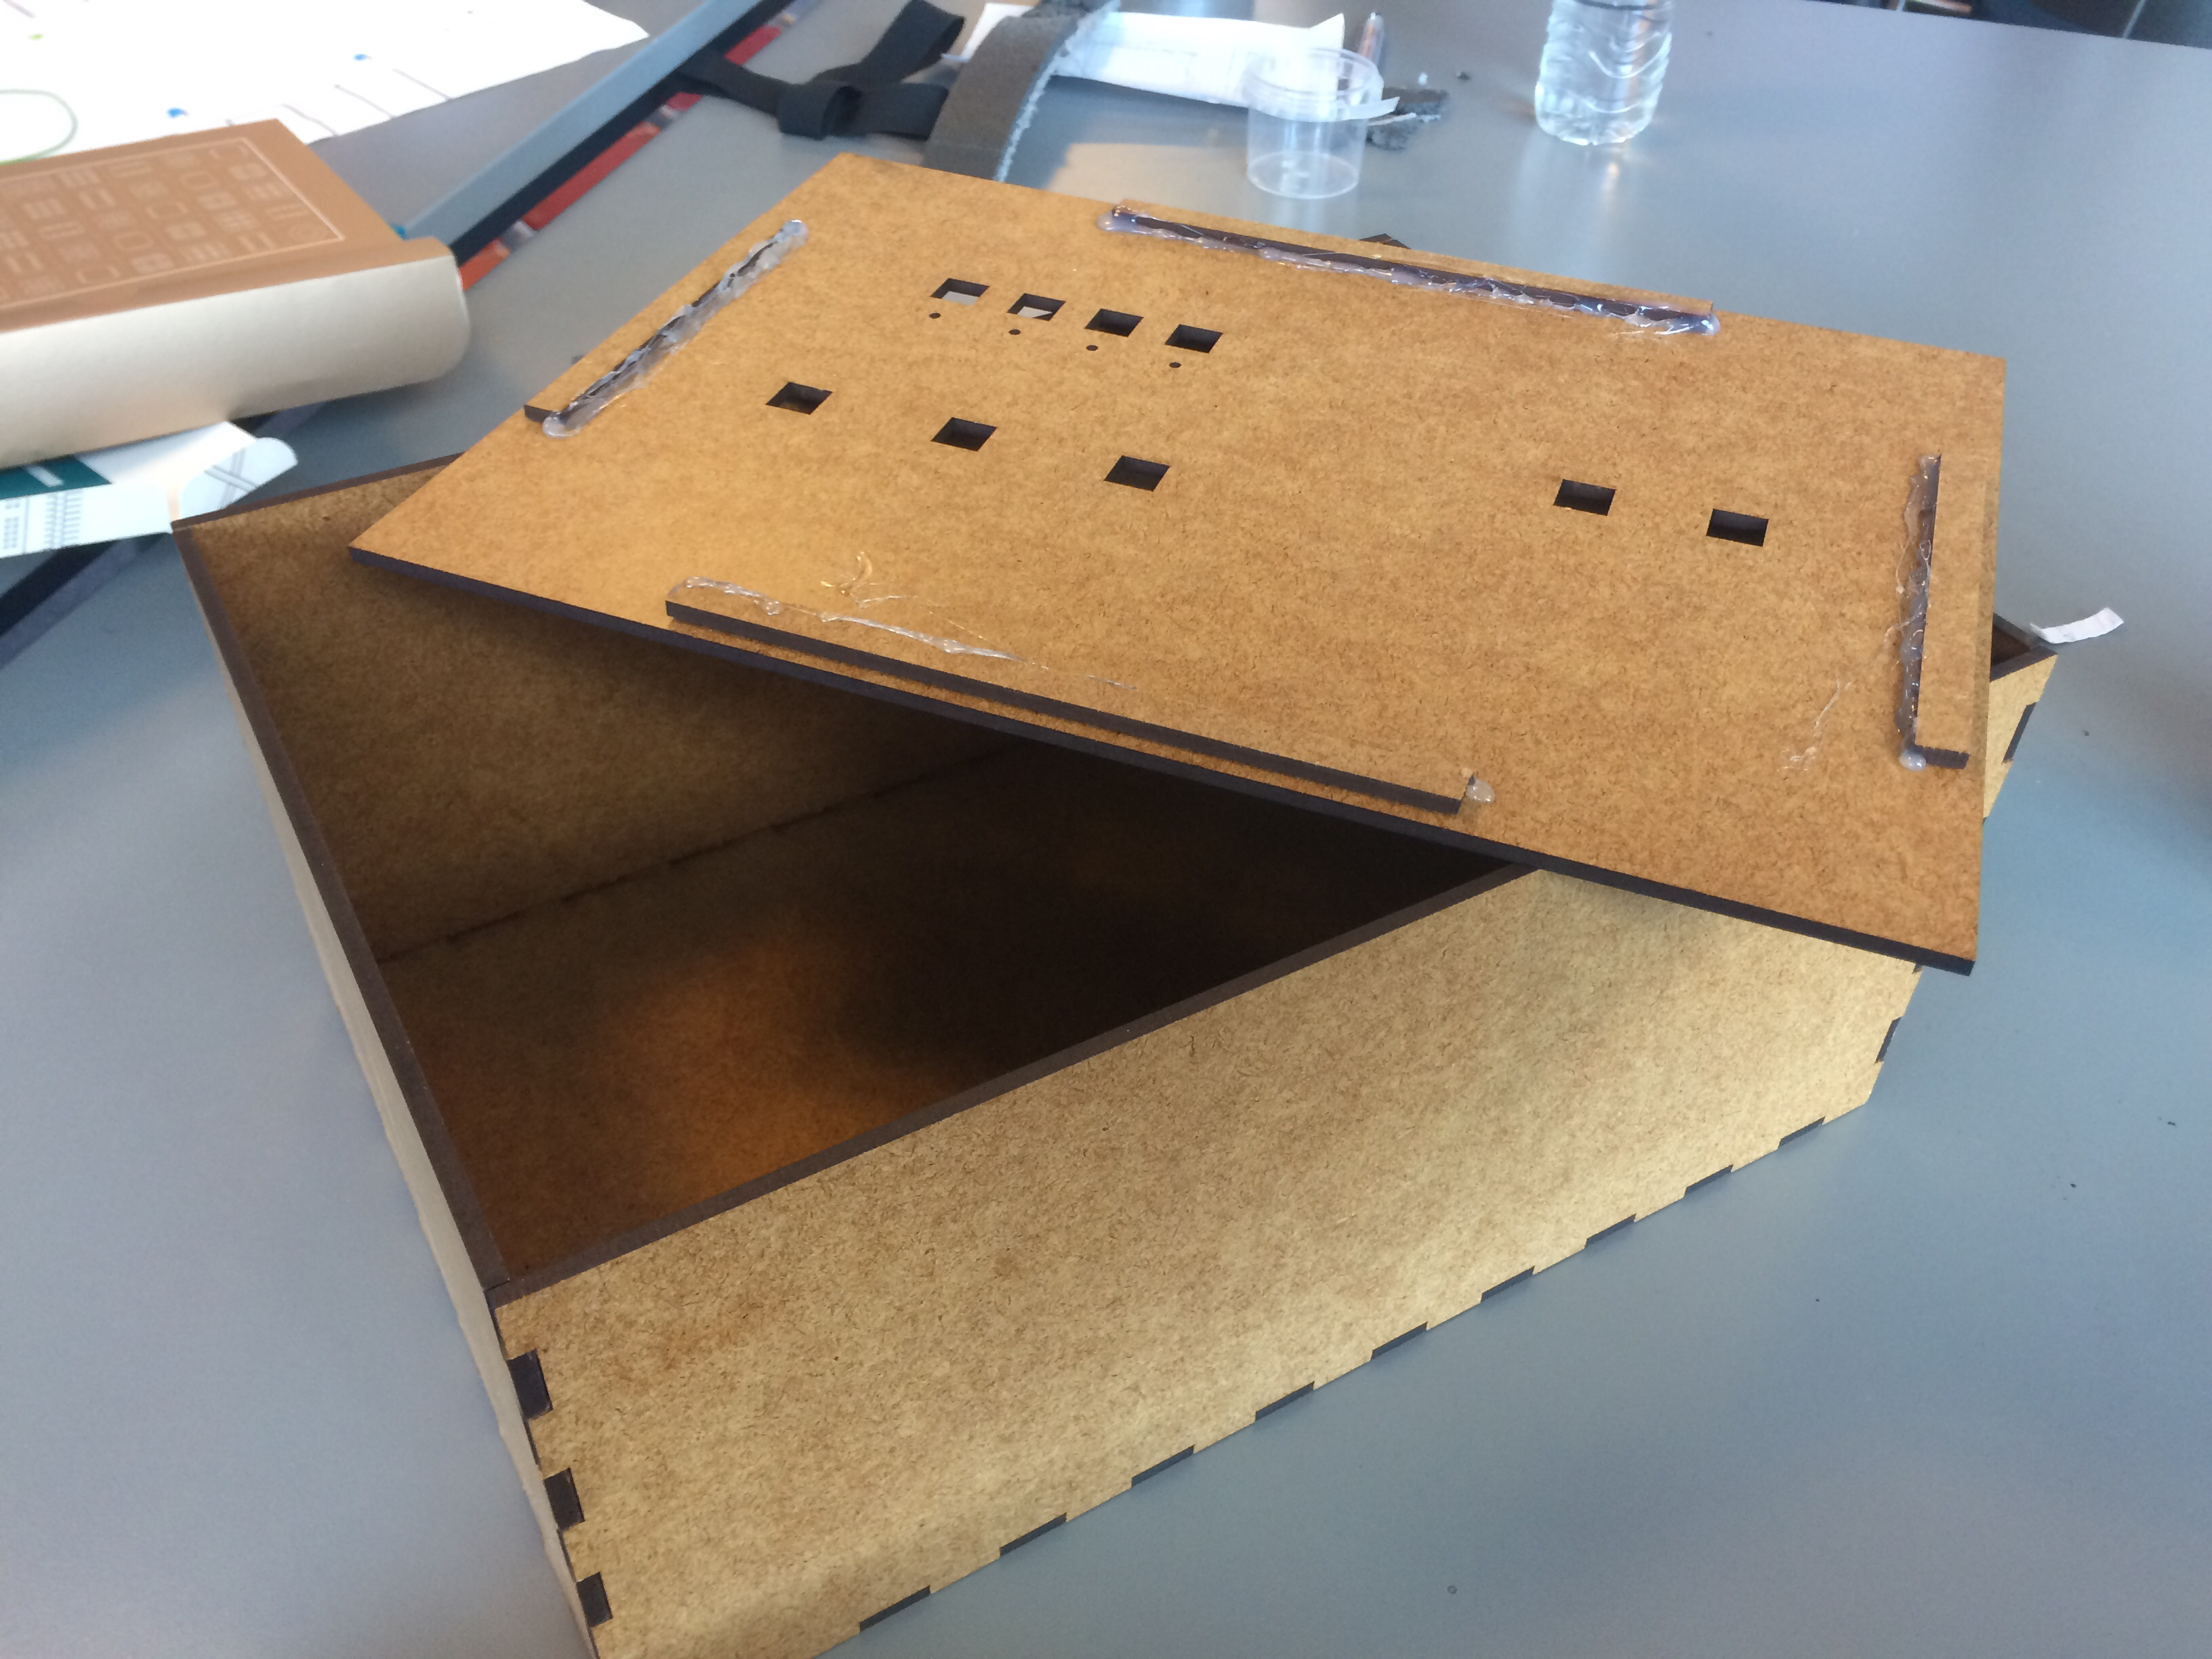
\includegraphics[width=0.7\linewidth]{figure/Design/finalbox2}
			\caption{The final prototype box}
			\label{fig:finalbox2}
		\end{figure}
		
		\begin{figure}[H]
			\centering
			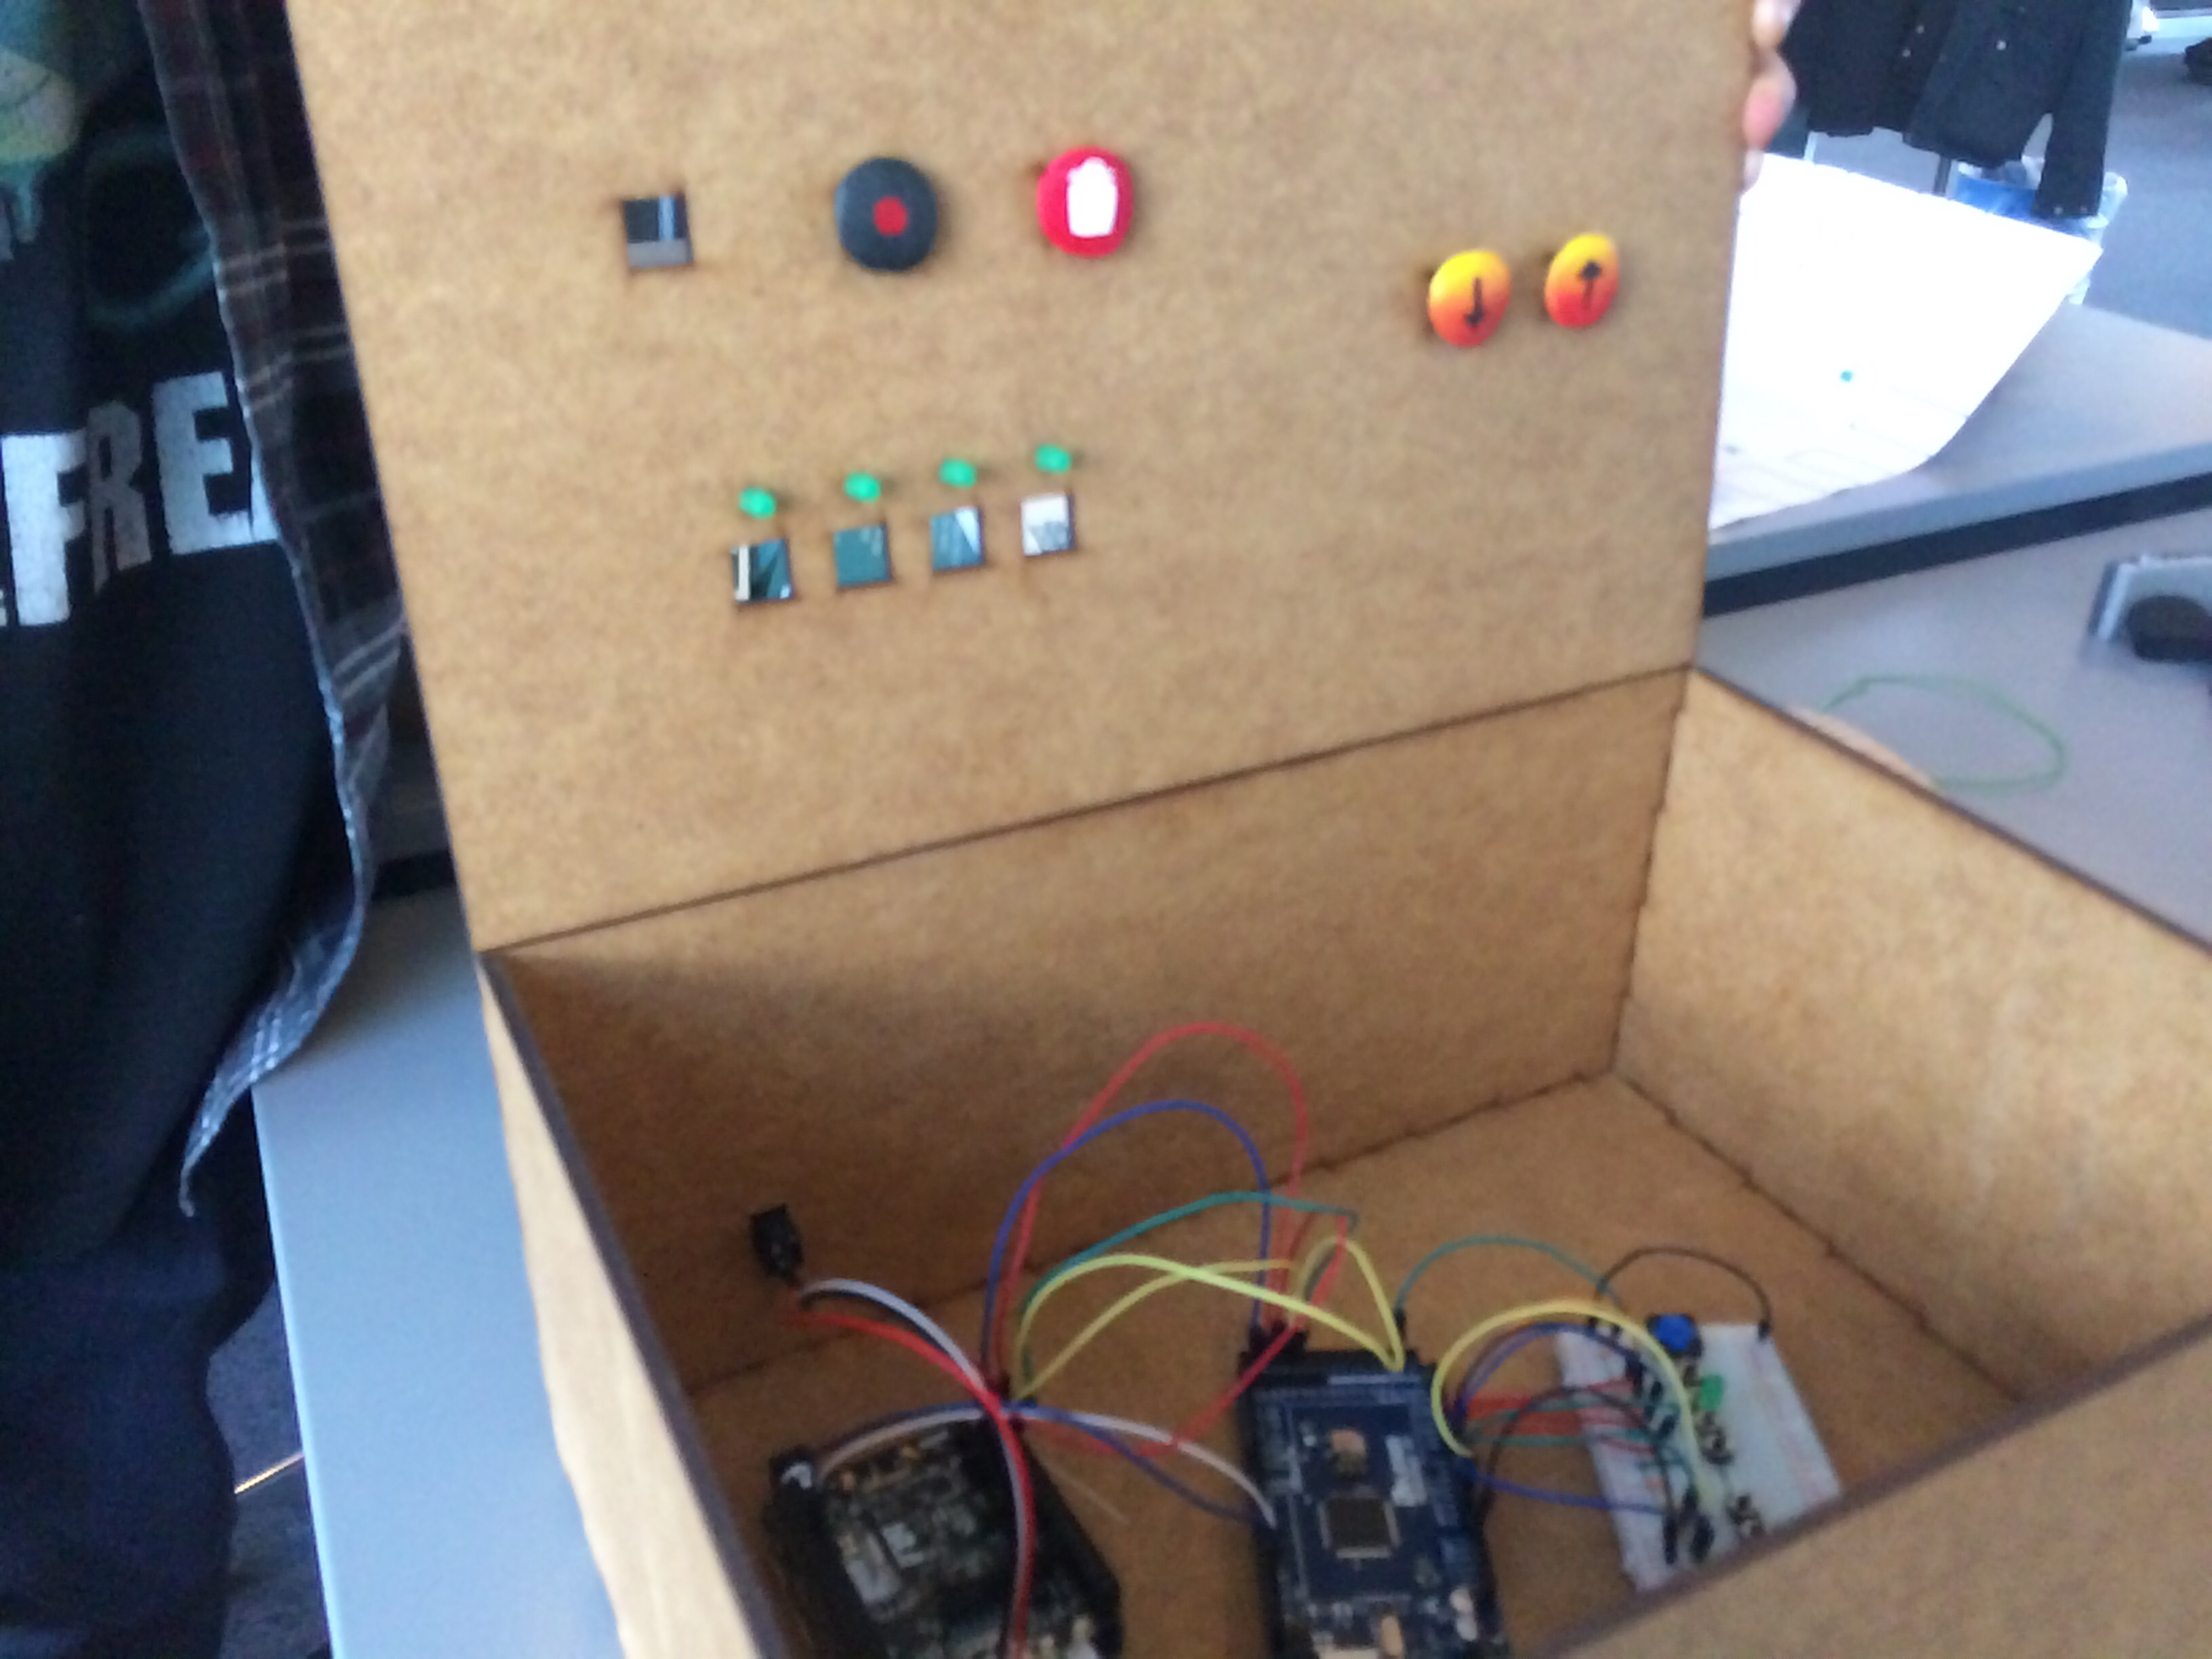
\includegraphics[width=0.7\linewidth]{figure/Design/finalbox3}
			\caption{The final prototype box with the electronic components inside}
			\label{fig:finalbox3}
		\end{figure}

\section{The mat}%Daniel

\section{Circuit}